\documentclass[twocolumn]{article}

\usepackage[english]{babel} 


\usepackage[utf8]{inputenc}
\usepackage[T1]{fontenc}
\usepackage{lmodern}
\usepackage{amsmath}
\usepackage{verbatim}
\usepackage{amssymb}
\usepackage{mathtools}
\usepackage{enumitem}
\usepackage{float}
\usepackage{titlesec} 

\titleformat{\subsection}[runin]{\normalfont\large\bfseries}{\thesubsection}{1em}{}

\setlength{\parindent}{0pt}

\begin{document}

\begin{center}

\Large{\textbf{MLDS: Homework 7}} \\
\textsc{\large{Andraž De Luisa}} \\
\vspace{6pt}
\small{\today}

\end{center}

\paragraph{} We apply Bayesian Logistic regression to a basketball shots dataset and infer the relationship between the input variables (angle and distance) and shot success. The input variables are normalized before inference.

\paragraph{} Before doing any computations, from a basic knowledge of basketball we can reason about the influence of the distance from the basket on the shot result. The coefficient beta for distance must be negative, if we want a probabilistic opinion about its distribution we could try to describe it with a (minus) gamma distribution.

\paragraph{} After a MCMC based inference (on the full dataset and on a size 50 random subset), we sample 20 000 coefficient pairs from the posterior distributions. The sampled distributions are shown in figure \ref{fig:scatter}. Both distributions' shapes are similar, but they differ in the means and variances. The coefficients, sampled from the model inferred on the subset have a much higher variance (note a high ratio of the samples having a positive distance coefficients, which is in contrast with our prior opinion).

\begin{figure}[ht]
    \centering
    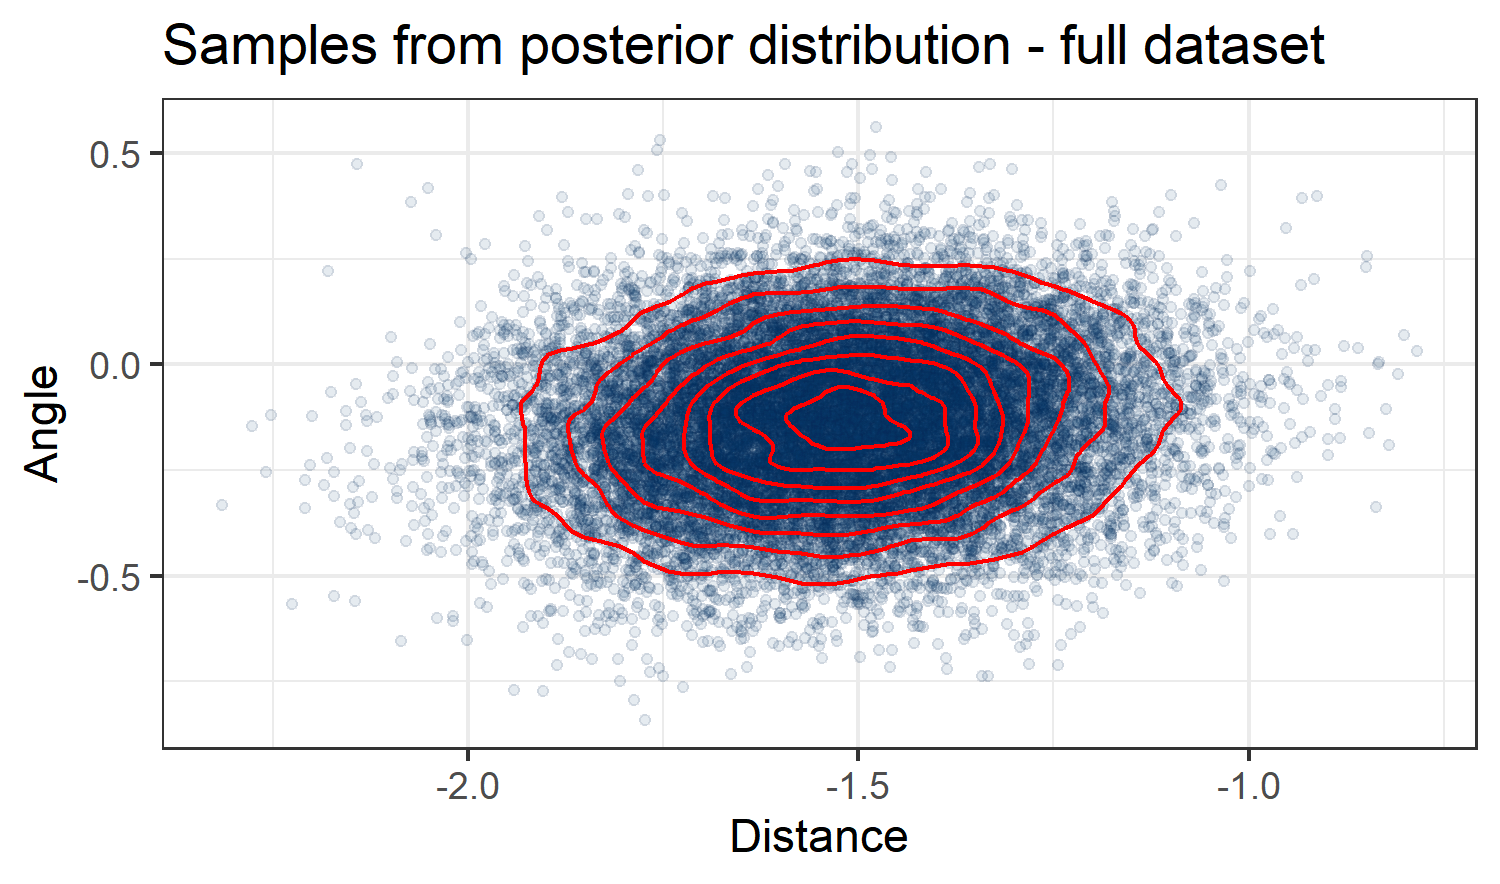
\includegraphics[width=.49\textwidth]{full.png}
    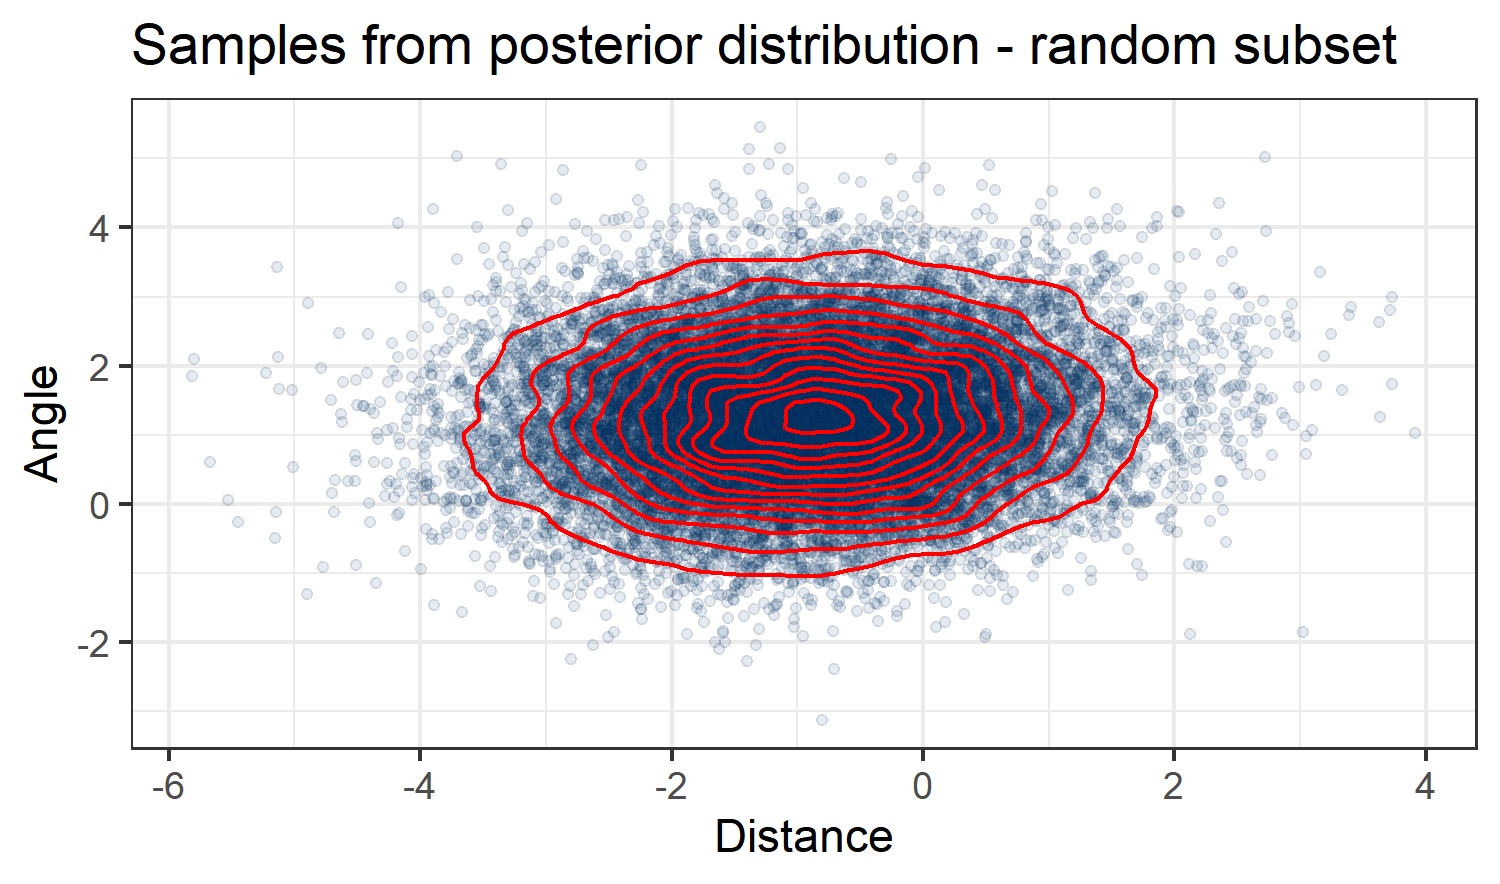
\includegraphics[width=.49\textwidth]{subset.png}
    \caption{Scatter plots with contours of the posterior samples of the angle and distance coefficients, sampled from an inferred model on the whole dataset and from a random subset of size 50. Note the different scales of the axis.}
    \label{fig:scatter}
\end{figure}

\paragraph{} We are interested in which variable is more important for the outcome of the shot (since both variables are normalized, the problem translates into which coefficient has a bigger absolute value). We estimate it with just counting the sampled instances in which the distance is bigger in the absolute value than the angle. For the samples, drawn from the model inferred on the whole dataset, the distance is almost surely more important than the angle (with the estimated probability 1).

\paragraph{} We are also interested in the influence of the angle variable to the shot success (positive or negative). Here we need just the marginal distribution of the angle coefficient. We compute a 95\% confidence interval $CI = [-0.49,\ 0.22]$. Since 0 is inside the CI, we might conclude that the angle doesn't have any influence on the shot success.

\end{document}